\chapter{Design}

\section{Overall System Design}

\subsection{Short description of the main parts of the system}
my system will consist of 5 main parts, using this information i have given a short description of what the system is meant to do:
\begin{itemize}
\item Log in window 
\begin{itemize}
\item this will display a login window and the central widget has input boxes for the user to input there user name and password
\item checks in the pharmacy's database to find if the user is registered to the system and has prority to enter the database.
\item the system then checks the users name and finds the password registered to that user. if the password entered is not the same the user will be asked to renter the password after the input box has been cleared.
\end{itemize}
\item Database display
\begin{itemize}
\item once the user has been accepted into the database the stock will come up on screen for the user 
\item the system will then check the stock to see if the amount of items is up to the minimum level and if the stock isn't to the minimum level then the system begins to request for more stock.
\item if the system find's an error e.g. missing stock or calculation problem it will give an error report to the user.
\end{itemize}
\item stock order form
\begin{itemize}
\item if the system find's a product low the system will bring up a order request form which will be sent to the warehouse.
\item
\end{itemize}
\end{itemize}
\subsection{System flowcharts showing an overview of the complete system}
\begin{figure}[H]
\centering
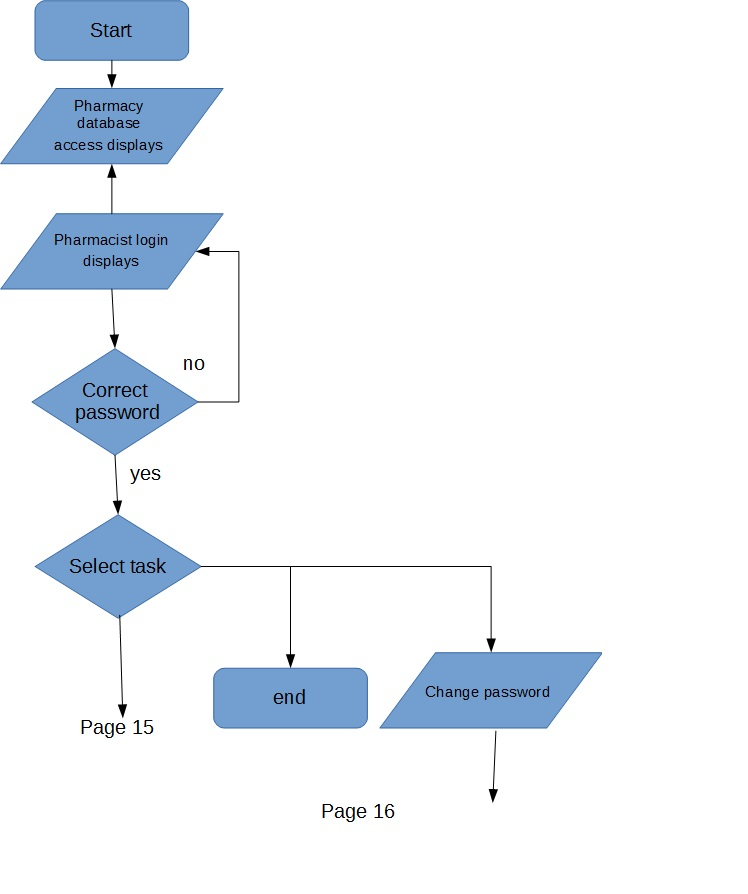
\includegraphics[width=140mm, scale=2]{system flow 1.JPG}
\end{figure}
\begin{figure}[H]
\centering
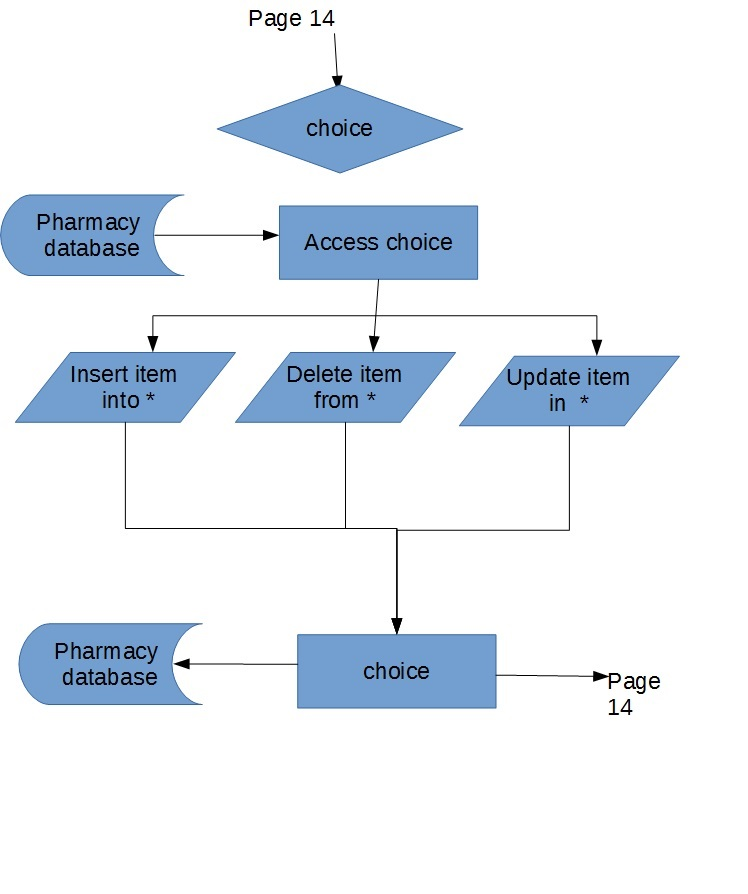
\includegraphics[width=140mm, scale=2]{system flow 2.JPG}
\caption{system flow \label{overflow}}
\end{figure}
\section{User Interface Designs}

\section{hardware specification}

\section{Program Structure}

\subsection{Top-down design structure charts}

\subsection{Algorithms in pseudo-code for each data transformation process}

\subsection{Object Diagrams}

\subsection{Class Definitions}

\section{Prototyping}

\section{Definition of Data Requirements}

\subsection{Identification of all data input items}

\subsection{Identification of all data output items}

\subsection{Explanation of how data output items are generated}

\subsection{Data Dictionary}
\begin{table}[H]
\begin{tabular}{|l|l|l|}
\hline
Data & Uses & Name \\
\hline
stock detail & stock number & stock check\\
\hline
prescription information & mediction needed & prescription\\
\hline
enough item in stock False & order more item & update stock\\
\hline
\end{tabular}
\end{table}

\subsection{Identification of appropriate storage media}

\section{Database Design}

\subsection{Normalisation}

\subsubsection{ER Diagrams}
\begin{figure}[H]
\centering
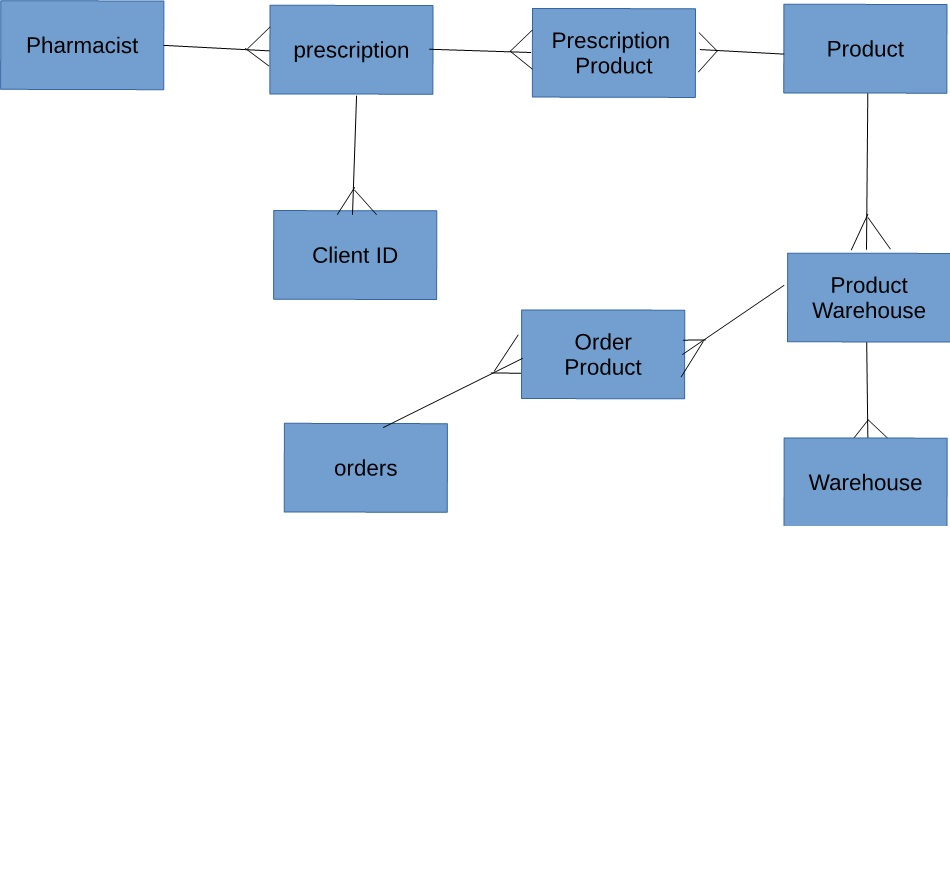
\includegraphics[trim = 0mm 100mm 0mm 0mm, clip, width=140mm, scale=2]{ERdiagram.JPG}
\caption{ERdiagram \label{overflow}}
\end{figure}
\subsubsection{Entity Descriptions}
\begin{itemize}
\item Client(\underline{clientID}, FirstName, surname, ClientPhoneNumber, Town, streetName,HouseNumber/name,Postcode)
\item Product(\underline{ProductID},ProductName, ProductWeight, ProductCode, Manufacturer, Price)
\item Pharmacist(\underline{PharamacistID}, PharmacistNum, Pharmacistname,
PharmacistEmail, PharmacistTown, PharmacistStreet, PharmacistPostcode)
\item Warehouse(\underline{WareHouseNum}, WarehouseTown, WarehouseStreet, WarehousePostcode)
\item PrescriptionCode(\underline{PrescriptionCode}, \emph{PharmacistID}, \emph{ClientID}, QuantityOfMed)
\item Order(\underline{OrderNum}, \emph{WareHouseNumber}, \emph{ProductID}, OrderDate, size)
\item Product on prescription(\underline{PrescritionProduct}, \emph{ProductID}, \emph{PrescritionCode})
\item product delivered from warehouse(\underline{ProductWareHouse}, \emph{ProductID}, \emph{WareHouseNumber})
\item Product ordered (\underline{OrderProduct}, \emph{ProductWareHouse}, \emph{Order})


\end{itemize}
\subsubsection{UNF}
\begin{table}[H]
\begin{tabular}{|l|}
\hline
\underline{Un-Normalised}\\
\hline
ClientID           \\
PharmacyNum        \\
Surname            \\
Firstname          \\
ClientPhoneNumber  \\
ClientAddress      \\
Postcode           \\
PrescriptionCode   \\
PharmacistID       \\
PharmacistTown     \\
PharmacistStreet   \\
PharmacistPostcode \\
PharmacistEmail    \\
PharmacyAddress    \\
PharmacyPhoneNumber\\
OrderNum           \\
OrderDate          \\
size               \\
ProductCode        \\
QuantityOfMed      \\
Weight             \\
ProductName        \\
Manufacturer       \\
Price              \\
Town               \\
Postcode           \\
StreetName         \\
HouseNumber/Name   \\
WareHouseNumber    \\
WareHouseStreet    \\
WareHouseTown\\
WarehousePostcode\\
\hline
\end{tabular}
\end{table}

\subsubsection{1NF to 3NF}
\underline{1NF}
\begin{table}[H]
\begin{tabular}{|l|l|}
\hline
\textbf{non-repeating} & \textbf{repeating} \\
\hline
\underline{PharmacyNum}&\underline{\underline{ClientID}}\\\hline
 OrderDate             &\underline{ \underline{PharmacyNum}} \\\hline
 OrderNum              & FirstName          \\\hline
 Pharmacystreet        & Surname            \\\hline
 PharmacyTown          & ClientPhoneNumber  \\\hline
 PharmacyPostcode      & Town               \\\hline
                       & Postcode           \\\hline
							  & HouseNumber/Name   \\\hline
							  & StreetName         \\\hline
                       & ProductCode        \\\hline
						     & QuantityOfMed      \\\hline
                       & ProductWeight      \\\hline
                       & ProductName        \\\hline
							  & PrescriptionCode   \\\hline
  							  & Manufacturer       \\\hline
							  & Price              \\\hline
&size\\\hline
&PharmacistName\\\hline
&PharmacistNumber\\\hline
&PharmacistTown     \\\hline
&PharmacistStreet   \\\hline
&PharmacistPostcode \\\hline
&WarehouseNumber\\\hline
&WarehouseTown \\\hline
&WarehouseStreet\\\hline
&WarehousePostcode\\\hline
\end{tabular}
\end{table}

\underline{2NF}
\begin{table}[H]
\begin{tabular}{|l|l|}
\hline
\textbf{repeating} & \textbf{Non repeating}\\
\hline
\underline{\underline{ClientID}}     &\underline{PharmacyNum} \\\hline
\underline{\underline{PharmacyNum}}  & OrderDate \\\hline
PrescriptionCode                     & Size\\\hline
                                     & OrderNum\\\hline
\underline{ClientID}                 & PharmacyStreet\\\hline
FirstName                            & PharmacyTown\\\hline
Surname                              & PharmacyPostcode\\\hline
ClientPhoneNumber                    & PharmacyPhoneNumber \\\hline
HouseNumber/Name         & \\\hline
Town                     & \\\hline
Postcode                 & \\\hline
StreetName               & \\\hline
 & \\\hline
\underline{PharmacyNum}  &\\\hline
PharmacistNumber         &\\\hline
PharmacistName           &\\\hline
PharmacistEmail          &\\\hline
PharmacistTown           &\\\hline
PharmacistStreet         &\\\hline
PharmacistPostcode       &\\\hline
QuantityOfMed            &\\\hline
ProductName       & \\\hline
ProductWeight     & \\\hline
ProductCode       & \\\hline
Manufacturer      & \\\hline
Price             & \\\hline
WarehouseTown &\\\hline
WarehouseStreet &\\\hline
WarehousePostcode&\\\hline
\end{tabular}
\end{table}

\underline{3NF}
\begin{table}[H]
\begin{tabular}{|l|l|l|l|}
\hline
\begin{tabular}{l}
\underline{ClientID}     \\
FirstName                \\
Surname                  \\
ClientPhoneNumber        \\
HouseNumber/Name         \\
Town                     \\
Postcode                 \\
StreetName               \\
\end{tabular}&
\begin{tabular}{l}
\underline{ProductID}\\
 ProductName        \\
 ProductWeight      \\
 ProductCode        \\
 Manufacturer       \\
 Price              \\
\end{tabular}&
\begin{tabular}{l}
\underline{OrderNumber}\\
\emph{WareHouseNumber}\\
\emph{ProductID}\\
 OrderDate\\
 Size\\
\end{tabular} &
\begin{tabular}{l}
\underline{PharmacistID} \\
PharmacistNumber         \\
PharmacistName           \\
PharmacistEmail          \\
PharmacistTown           \\
PharmacistStreet         \\
PharmacistPostcode       \\
\end{tabular} \\
\hline
\begin{tabular}{l}
\underline{PrescriptionCode} \\
\emph{PharmacistID} \\
\emph{clientID}\\
 QuantityOfMed            \\
\end{tabular}&
\begin{tabular}{l}
\underline{WareHouseNumber}\\
WarehouseTown \\
WarehouseStreet \\
WarehousePostcode\\
\end{tabular}&
\begin{tabular}{l}
\underline{PrescritionProduct}\\
\emph{ProductID}\\
\emph{PrescritionCode}\\
\end{tabular}&
\begin{tabular}{l}
\underline{ProductWareHouse}\\
\emph{ProductID}\\
\emph{WareHouseNumber}\\
\end{tabular}\\\hline
\begin{tabular}{l}
\underline{OrderProduct}\\
\emph{ProductWareHouse}\\
\emph{Order}\\
\end{tabular}&
\begin{tabular}{l}
\underline{Manufacturer}\\
ManufacturerPostcode\\
ManufacturerStreet\\
ManufacturerTown\\
\end{tabular}&
\begin{tabular}{l}
\end{tabular} &
\begin{tabular}{l}
\end{tabular}\\
\hline
\end{tabular}
\end{table}
\section{Security and Integrity of the System and Data}

\subsection{Security and Integrity of Data}


\subsection{System Security}

\section{Validation}

\section{Testing}

\begin{landscape}
\subsection{Outline Plan}

\begin{center}
    \begin{tabular}{|p{2cm}|p{5cm}|p{5cm}|p{4cm}|}
        \hline
        \textbf{Test Series} & \textbf{Purpose of Test Series} & \textbf{Testing Strategy} & \textbf{Strategy Rationale}\\ \hline
        Example & Example & Example & Example \\ \hline
    \end{tabular}
\end{center}

\subsection{Detailed Plan}

\begin{center}
    \begin{longtable}{|p{1.5cm}|p{2.5cm}|p{2.5cm}|p{2cm}|p{2cm}|p{2cm}|p{2cm}|p{2cm}|}
        \hline
        \textbf{Test Series} & \textbf{Purpose of Test} & \textbf{Test Description} & \textbf{Test Data} & \textbf{Test Data Type (Normal/ Erroneous/ Boundary)} & \textbf{Expected Result} & \textbf{Actual Result} & \textbf{Evidence}\\ \hline
        Example & Example & Example & Example & Example & Example & Example & Example \\ \hline
    \end{longtable}
\end{center}
\end{landscape}
